\documentclass{beamer}

\usepackage{graphicx}
\usepackage{caption}
\usepackage{subcaption} % for subfigure
\usepackage{hyperref}
\usepackage{amssymb}
\usepackage{tabularx}
\usepackage{multicol}
\usepackage{algpseudocode}
\usepackage{amsthm} % for theorem
\usepackage{algorithm}
\usetheme{Warsaw}
\title[Optimizing Join Enumeration] % (optional, only for long titles)
{Optimizing Join Enumeration in Transformation-based Query Optimizers}
\subtitle{BTP Presentation}
\author[Anil Shanbhag] % (optional, for multiple authors)
{
Anil Shanbhag \\
Roll No: 100050082 \\
}
\institute[Universitäten Hier und Dort] % (optional)
{
	
}
\date[KPT 2004] % (optional)
{
Guide: Prof. S. Sudarshan \\
}
\subject{Informatik}


\begin{document}
\frame{\titlepage}
\begin{frame}

\frametitle{Outline}
\begin{itemize}
\item Introduction to Query Optimization
\item Related Work
\item Evaluate existing rule sets
\item Rule set RS-B3
\item N-ary Join Rule
\end{itemize}
\end{frame}

  \begin{frame}
    \frametitle{Introduction to Query Optimization}
    \tableofcontents[Introduction to Query Optmization]

Queries submitted to database are typically in high-level language. The goal of query optimization it to find the most-efficient way to execute the given query. Query optimizers typically follow a three step approach:
\begin{itemize}
	\item  Generate all execution plans that are logically equivalent to the user-submitted query.
	\item Estimate the cost of executing each of the alternate plans.
	\item Search through the space of all generated plans to find the plan with least cost.
\end{itemize}
  \end{frame}
  
  \begin{frame}
    \frametitle{Space of Logically Equivalent Plans}
The steps involved in generating the space of logically equivalent plans :
\begin{itemize}
	\item Query is parsed to generate a query tree
	\item Logical Query DAG is constructed from the query tree.
	\item Expand the LQDAG using transformation rules to encompass the space of all equivalent logical plans. This is called Logical Plan Space.
	\item The implementation of logical operators is not defined, adding the different implementations for each operator we get the Physical Plan Space.
\end{itemize}
	\end{frame}
	\begin{frame}
	\frametitle{Example}
    \begin{figure}[here]
\begin{center}
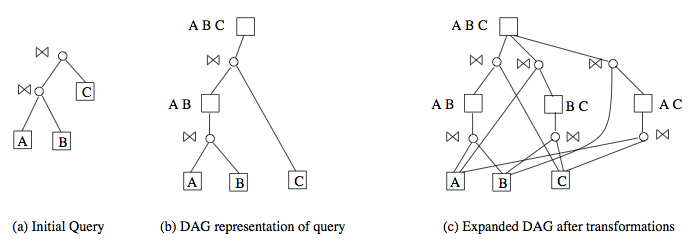
\includegraphics[width=10cm]{Figures/example_logical.png}
\end{center}
\caption{Logical Plan Space Generation for $A \bowtie B\bowtie C$}
\label{fig:joinabc}
\end{figure}
  \end{frame}

  \begin{frame}
  \frametitle{Motivation}
  \begin{itemize}
  \item Long ago, Ono and Lohman gave a lower bound of $O(3^n)$ with n the number of relations, on the complexity join enumeration.
  \item Exhaustive search is computationally expensive.
  \item \textit{Heuristic}: Consider all possible bushy join trees, but exclude trees with cross products from the search (presuming that all considered queries span a connected query graph)
  \item Interesting work lately on bottom-up dynamic programming and top-down memoization based join enumeration algorithms that achieve the lower bound and explore the reduced space effectively.
  \item On the other hand, transformation-based optimizers generate exponential number of duplicates.  
  \end{itemize}
  \end{frame}
  \begin{frame}
\frametitle{Problem Statement}
The question is can join enumeration in transformation-based query optimizers be as efficient as in DP/memoization based join optimizers ? 

Starting from a connected query tree, our goal is to 
\begin{itemize}
	\item Generate the space of all join trees without cross products
	\item Always be within the space 
	\item Avoid generation of duplicates
\end{itemize}
  \end{frame}
  
% RELATED WORK %
  \begin{frame}
  \frametitle{TreeOpt Algorithm}
  \framesubtitle{Related Work}
Finding a solution for general graphs is NP-Hard, however for tree queries ie: queries whose join graphs form a tree for nested loop join, it is possible to find the optimal solution in polynomial time. \vspace{\baselineskip}

Cost function f satisfies \textit{adjacent sequence interchange} property if there exists a rank function $r_{f}$ such that $f(AS_{1}S_{2}B) <= f(AS_{1}S_{2}B)$ if and only if $r_{f}(S_{1}) <= r_{f}(S_{2})$. If yes, optimal sequence can be found in $O(n log(n))$ where the order constraints are series parallel. \vspace{\baselineskip}

We call TreeOpt once with each node as root. In this case, the order constraints form directed tree which is a special case of series parallel constraints. 
\end{frame}
\begin{frame}
\frametitle{TreeOpt Algorithm Contd.}
  \framesubtitle{Related Work}
\begin{algorithm}[H]
  \caption{Finding Optimal Nesting Order for Tree Queries
    \label{alg:treeopt}}
	\begin{algorithmic}[1]
	\Function{TreeOpt}{$T,R$}
		\State $rt \gets$ directed tree rooted at R   
		\While {$rt$ is not a chain}
			\State Find a wedge in the tree $rt$
			\State Apply \textsc{Normalize} to each chain of the wedge.
			\State Merge the two chains into one by ordering the nodes by their ranks.		
		\EndWhile
	\EndFunction
  \end{algorithmic}
\end{algorithm}
  \end{frame}

  \begin{frame}
  \frametitle{FAB Algorithm}
  \framesubtitle{Related Work}
 \textsc{TreeOpt} generates optimal plan for any acyclic join graph in polynomial time. However for cyclic queries, it does a bad job at even producing a near optimal plan. \vspace{\baselineskip}
 
FAB approach uses a global-impact based ordering, in which the global impact of each relation explored and used to decide the ordering. The global impact of a  relation $R_{i}$ is the product of the size of all other relations and join selectivity not related to $R_{i}$. Intuitively if node $R_{i}$ has least impact, it means that it itself has a combination of large size and low join selectivity. The FAB algorithm picks the node with least impact and puts it as the last node to be joined. It then recalculates the impact of each node after removing the element from the join graph.

  \end{frame}

\begin{frame}
\frametitle{Top-Down Join Enumeration}
A generic top-down join enumerator first initializes the costs of the base relations and starting from join graph J, recursively explores the entire space. If the best tree for a graph is not known, a suitable partitioning strategy is used to partition $S$ into two sets $S_{1}$ and $S_{2}$ such that the following condition are satisfied :
\begin{itemize}
	\item $S_{1}$ with $S_{1} \subset S$ induces a connected subgraph $G_{|S_{1}}$
	\item $S_{2}$ with $S_{2} \subset S$ induces a connected subgraph $G_{|S_{2}}$
	\item $S_{1} \cup S_{2} = S$ and $S_{1} \cap S_{2} = \phi$
	\item $\exists (v_{1}, v_{2}) \in E$ | $v_{1} \in S_{1} \wedge v_{2} \in S_{2}$
\end{itemize}
If $(S_{1},S_{2})$ is valid, so is $(S_{2},S_{1})$. The set of all pairs $(S_{1},S_{2})$ such that symmetric pairs are counted only once is denoted by $P^{sym}_{ccp}(S)$.
\end{frame}

\begin{frame}
\frametitle{Top-Down Join Enumeration Contd.}
The recursive decent stops when $|S| = 1$ or the best tree is already known. Once all the possibilities have been tried, a subroutine \textsc{BuildTree} updates memotable $BestTree$ if a plan better than existing plan is found. After all $(S_{1}, S_{2}) \in P^{sym}_{ccp}(S)$ have been tried, the entry in $BestTree[S]$ corresponds the optimal join tree for set of relations in $S$.\vspace{\baselineskip}

Depending on the choice of partitioning algorithm, the overall performance of \textsc{TDPlanGen} can vary by orders of magnitude.
\end{frame}

\begin{frame}
\frametitle{Top-Down Join Enumeration Contd.}
\begin{figure}[here]
\begin{center}
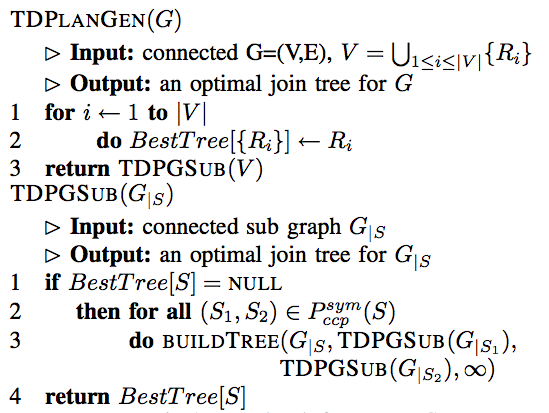
\includegraphics[width=9cm]{Figures/tdplangen.png}
\end{center}
\caption{Pseudocode for TDPLANGEN}
\label{fig:tdplangen}
\end{figure}
\end{frame}

% RULE SETS %
  \begin{frame}
  \frametitle{Rule set RS-B0}
  \framesubtitle{Analysing existing rule sets}
  \begin{itemize}
	\item Left Associativity \\ $A \bowtie (B \bowtie C) \rightarrow (A \bowtie B) \bowtie C$
	\item Right Associativity \\ ($A \bowtie B) \bowtie C \rightarrow A \bowtie (B \bowtie C)$
	\item Commutativity \\ $A \bowtie B \rightarrow B \bowtie A$
\end{itemize}

  Clearly the rules are redundant. We can remove either left-associativity or right-associativity and still explore the same space. We shall show completeness later.
  \end{frame}
  
  \begin{frame}
  \frametitle{Rule set RS-B1}
  \framesubtitle{Analysing existing rule sets}
\begin{itemize}
	\item Left Associativity \\ $A \bowtie (B \bowtie C) \rightarrow (A \bowtie B) \bowtie C$
	\item Commutativity \\ $A \bowtie B \rightarrow B \bowtie A$
\end{itemize}

Pellenkoft et al. have shown that RS-B1 leads to exponential number of duplicates. The number of duplicates generated during the construction of MEMO-structure encoding all bushy trees for a clique join graph on n relations is $4^{n}-3^{n+1}+2^{n+2}-n-2$.

We show later that this rule set is actually complete. Hence it is possible to explore the search space using rules.
  \end{frame}
  
  \begin{frame}
  \frametitle{Rule set RS-B2}
  \framesubtitle{Analysing existing rule sets}
\begin{itemize}
	\item $R_{1}$ : Commutativity \\ $A \bowtie_{0} B \rightarrow B \bowtie_{1} A$ \\
	Disable 	$R_{1}, R_{2}, R_{3}, R_{4}$ for application on new operator $\bowtie_{1}$
	\item $R_{2}$ : Left Associativity \\ $A \bowtie_{0} (B \bowtie_{1} C) \rightarrow (A \bowtie_{2} B) \bowtie_{3} C$ \\ 
	Disable 	$R_{2}, R_{3}, R_{4}$ for application  on new operator $\bowtie_{3}$	
	\item $R_{3}$ : Right Associativity \\ $(A \bowtie_{0} B) \bowtie_{1} C \rightarrow A \bowtie_{2} (B \bowtie_{3} C)$ \\
	Disable $R_{2}, R_{3}, R_{4}$ for application on new operator $\bowtie_{2}$	
	\item $R_{4}$ : Exchange \\ $(A \bowtie_{0} B) \bowtie_{1} (C \bowtie_{2} D) \rightarrow (A \bowtie_{3} C) \bowtie_{4} (B \bowtie_{5} D)$ \\
	Disable 	$R_{1}, R_{2}, R_{3}, R_{4}$ for application on new operator $\bowtie_{4}$
\end{itemize}  

   RS-B2 generates the space of all bushy join trees without duplicates.
  \end{frame}

  \begin{frame}
  \frametitle{Completeness of RS-B1}
  Problem: Given a connected join graph J and query tree Q, show that using RS-B1 we can reach any other valid query tree Q' from Q while remaining in cross-product free space.  \vspace{\baselineskip}
  
  Reduction 1: Sufficient to show  one route between Q and Q'. The route we show is Q to valid left deep tree to Q'. \vspace{\baselineskip}
  
  Choice of left deep tree: Given the input join graph $J$ is completely connected we can number the nodes $1,2...n$ such that $(..(R_{1}\bowtie R_{2})...)\bowtie R{n}$ is a valid left-deep join tree. \vspace{\baselineskip}
  
  Reduction 2: If in $Q$ we can pull up $R_{n}$ so that its the last relation to be joined, we are done.
  
  \end{frame}
  
  \begin{frame}
  \frametitle{Completeness of RS-B1 Contd.}
\begin{minipage}{\textwidth}
\begin{columns}[T]
\begin{column}{0.55\textwidth}
We can reduce the given tree to reduced query tree as shown on right. Height of tree is defined in conventional sense. \vspace{\baselineskip}

Reduction 3: If we can pull $R_k$ one level up ie: reduce the height of reduced query tree by one, we are done. \vspace{\baselineskip}
\end{column}
\begin{column}{0.45\textwidth}
\begin{figure}[here]
\begin{center}
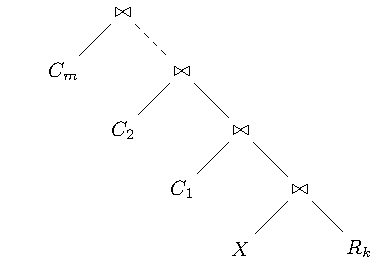
\includegraphics[width=5cm]{Figures/rsb1-proof.pdf}
\end{center}
\caption{Reduced Query Tree}
\label{fig:rsb1-proof}
\end{figure} 
\end{column}
\end{columns}
\end{minipage}

  \end{frame}

  \begin{frame}
  \frametitle{Completeness of RS-B1 Contd.}
  To prove reduction 3: The bases case m = 0 holds trivially. For m $>$ 0, since $R_{k}$ was the last relation to be joined, there exists some $C_i$ which has an edge with X. We pull down $C_i$ using  $C \rightarrow LA \rightarrow C$. Finally $X \bowtie C_i$ and renamed as new $C_{i'}$. Height of tree reduced by 1. \vspace{\baselineskip}
  
  Finally for the other direction ie: from left-deep tree to Q', it is equivalent to using rules right associativity and commutativity and going from the join tree to left-deep tree. Right associativity can be done using a sequence of left associativity and commutativity : $RA \Rightarrow C \rightarrow C \rightarrow LA \rightarrow C$. \vspace{\baselineskip}
  
  Hence Proved :-)
  \end{frame}
  
  \begin{frame}
  \frametitle{Incompleteness of RS-B2}
  Consider a simple example. Given a set of relations to be joined with join graph J and initial query tree Q, we wish to go to Q'. However using RS-B2 it is not possible as it would lead to formation of subtree $R_2 \bowtie R_3$ which has cross product.
\begin{figure}[ht]
\centering
\begin{subfigure}[b]{0.24\linewidth}
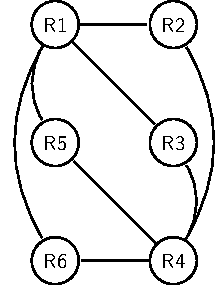
\includegraphics[width=2cm]{Figures/rsb2-predicates.pdf}
\caption{Join Graph J}
\label{fig:rsb2-counter}
\end{subfigure}
\begin{subfigure}[b]{0.35\linewidth}
	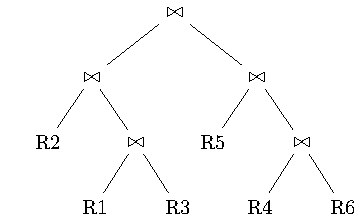
\includegraphics[width=3.5cm]{Figures/rsb2-counter.pdf}
\caption{Query Tree $Q$}
\label{fig:minipage1}
\end{subfigure}
\begin{subfigure}[b]{0.35\linewidth}
	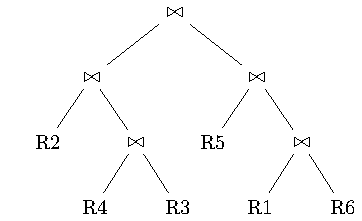
\includegraphics[width=3.5cm]{Figures/rsb2-counter2.pdf}
\caption{Query Tree $Q_{2}$}
\label{fig:minipage2}
\end{subfigure}
\end{figure}

  \end{frame}
  
  \begin{frame}
  \frametitle{Rule set RS-B3}
\begin{itemize}
	\item $R_{1}$: Commutativity \\ $A \bowtie_{0} B \rightarrow B \bowtie_{1} A$ \\
	Disable $R_{1}$,$R_{2}$ for application on new operator $\bowtie_{1}$
	\item $R_{2}$: Right Associativity \\ $(A \bowtie_{0} B) \bowtie_{1} C \rightarrow A \bowtie_{2} (B \bowtie_{3} C)$ \\
	Disable $R_{1}$,$R_{2}$ for application on new operator $\bowtie_{2}$. Enable $R_{3}$ for application on new operator $\bowtie_{2}$.		
	\item $R_{3}$: Left Associativity \\ $A \bowtie_{0} (B \bowtie_{1} C) \rightarrow (A \bowtie_{2} B) \bowtie_{3} C$ \\
	Enable $R_{1}$ for application on new operator $\bowtie_{3}$.
\end{itemize}
  \end{frame}
  
  \begin{frame}
  \frametitle{Completeness of RS-B3}
\begin{figure}[here]
\begin{center}
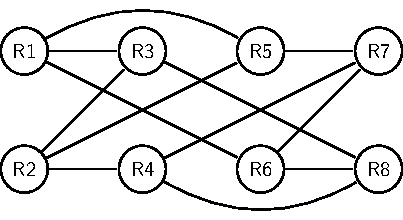
\includegraphics[width=5cm]{Figures/extreme.pdf}
\end{center}
\caption{Extreme case for RS-B3}
\label{fig:extreme}
\end{figure}
There exist edge cases. $Q = [R_{1}R_{2}R_{3}R_{4}]\bowtie[R_{5}R_{6}R_{7}R_{8}]$ and $Q' = [R_{1}R_{2}R_{5}R_{6}]\bowtie[R_{3}R_{4}R_{7}R_{8}]$. In the current scheme, it is not possible to do this. Also note that no locking constrains while restricting the number of times group of relations move around the join to 2 can achieve this. However the ray of hope is that using a small perturbation ie: moving $R_{4}$ to right hand side and then starting the enumeration will work.
  \end{frame}
  
  \begin{frame}
  \frametitle{Efficiency of RS-B3}
  The number of duplicates generated by \textbf{RS-B3} during the exploration of a class that combines k relations, on a completely connected graph is: $O(3^l2^r)$
  
  \begin{eqnarray*}
C &=& \sum\limits_{k=1}^{l-1} {l \choose k} A(k+r) \nonumber \\ 
 &=& \sum\limits_{k=1}^{l-1} {l \choose k} (2^{k+r} - 2) \nonumber \\
 &=& 2^r (3^l - 2^l - 1) - 2 (2^l - 2) \nonumber \\
 	D &=& 2 + 2*C - A(k) \nonumber \\
	  &=& 2 + 2^r (3^l - 2^l - 1) - 2 (2^l - 2) - (2^k - 2) \nonumber \\
	  &=& 3^l 2^r - 2^{k+1} - 2^r - 2^{l+1} +  8 \nonumber \\
\end{eqnarray*}
 D is the number of duplicates
  \end{frame}
  
\begin{frame}
\frametitle{Graph-based Join Enumeration}
DP-based and memoization-based enumeration algorithms by Pit Fender et al. and De Haan et al. for join enumeration are more efficient in comparison to transformation-based ones in that they are able to enumerate the entire space without generating duplicates. \vspace{\baselineskip}

We propose a new method of doing join enumeration in transformation-based optimizers based on ideas from memoization based join enumerators.
\end{frame}  
  
  \begin{frame}
  \frametitle{\textsc{MinCutConservative}}
The secret sauce of \textsc{TDMinCutConservative} is \textsc{MinCutConservative}.

\begin{figure}[here]
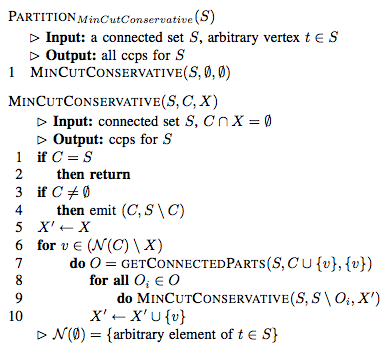
\includegraphics[width=7cm]{Figures/mincutconservative.png}
\caption{Pseudocode for \textsc{MinCutConservative}}
\label{fig:mincutconservative}
\end{figure}
  \end{frame}
  
\begin{frame}
\frametitle{N-ary Join Rule}
The \textsc{N-ary Join} rule generates all ccps for the given set of n-relations. It is in essence a vanilla coated \textsc{MinCutConservative} algorithm. \vspace{\baselineskip}

We store two additional sets at each equivalence node:

\begin{itemize}
	\item \textsc{EqSet} : A set of all combinations of base equivalence classes being joined to generate this equivalence class. Along with this we need to store the ids of join operators of a feasible join ordering for these base equivalence class. This is used to infer the join graph.
	\item \textsc{HSet} : A set of hashes. For every set of base equivalence class that we enumerate, we generate a hash and store it in the parent equivalence class as a proof that this set has been enumerated. This is to prevent repeated enumeration of the same set of base equivalence classes.
\end{itemize}
\end{frame}

\begin{frame}
\frametitle{N-ary Join Rule contd.}
When \textsc{N-ary Join} rule is applied at a logical join operator $op$ get the \textsc{EqSet} of the left child and right child. For all combination of $S=S_{1} \cup S_{2}$ where $S_{1}\in \textsc{EqSet}_{L}$ and $S_{2}\in \textsc{EqSet}_{R}$, generate $hash(S)$ and check to ensure it has not been enumerated before. It it has not been enumerated, call \textsc{MinCutConservative}$(G_{|S})$. For every ccp generated add a new operation node to $child(parent(op))$. For every new equivalence class generated, insert it as a left-deep tree got by doing a depth-first traversal on the join graph (such a tree exists as the graph induced by these base equivalence classes is connected).
\end{frame}

\begin{frame}

\Huge Thank You

\end{frame}
\end{document}